\documentclass[xcolor={table}]{beamer}

\usetheme{Dragonfly}

\title{Introduction to Haskell\\\& some category theory}
\subtitle{Wellington Functional Programming}
\projectcode{26 March 2015}
\author{Finlay Thompson}
\date{}

\AtBeginSection[]{
  \begin{frame}
  \vfill
  \centering
  \Huge
    \insertsectionhead\par%
  \vfill
  \end{frame}
}

\begin{document}

\titleslide

\section{Introduction}

\begin{frame}{}{}

    \begin{columns}
    \column{0.5\textwidth}
    {\Large Haskell is strange ? }

    \pause\bigskip
    A functional programming language

    \pause\bigskip
    With lazy evaluation
    
    \pause\bigskip
    Pure, with no side effects 
    
    \pause\bigskip
    Fairly old\pause, fairly odd

    \column{0.5\textwidth}
    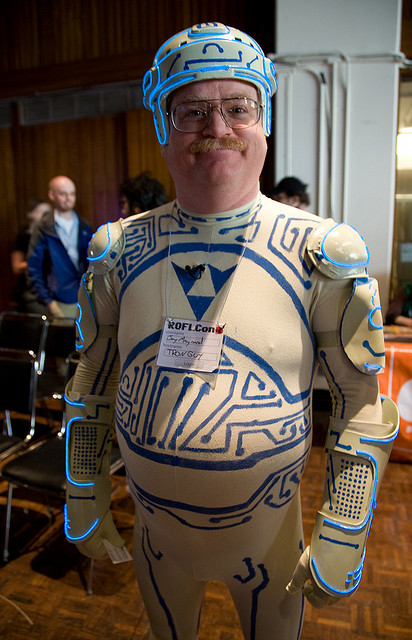
\includegraphics[width=0.9\textwidth]{images/tron-guy.jpg}
        
    \end{columns}

\end{frame}

\begin{frame}{}{}

    \begin{columns}
    \column{0.5\textwidth}
    {\Large Haskell is hard ?}

    \pause\bigskip
    My program won't compile,\\ and I don't know why ?

    \pause\bigskip
    The tutorials online are confusing.

    \pause\bigskip
    Oh god, I am reading math !

    \pause\bigskip
    Huh ?

    \column{0.5\textwidth}
    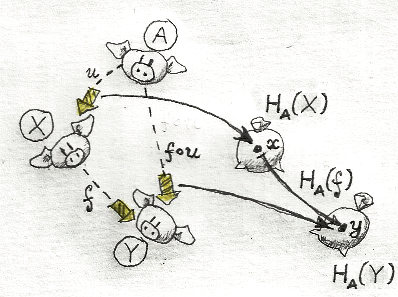
\includegraphics[width=0.9\textwidth]{images/content-proxy.png}
        
    \end{columns}

\end{frame}

\begin{frame}{}{}

    \begin{columns}
    \column{0.5\textwidth}
    {\Large Haskell is impractical ? }

    \pause\bigskip
    Strong type system gets in the way

    \pause\bigskip
    Hard to install, and find good libraries

    \pause\bigskip
    Impossible to find other developers

    \pause

    \column{0.5\textwidth}
    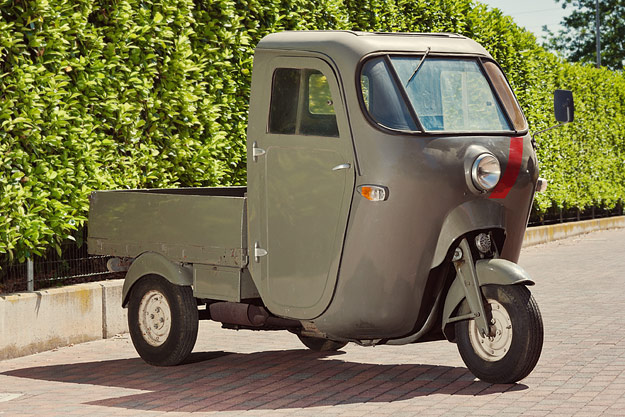
\includegraphics[width=0.9\textwidth]{images/ducati-muletto.jpg}
        
    \end{columns}

\end{frame}

\begin{frame}{}{}

    {\Large But, Haskell is awesome! }

    \pause
    Is Haskell weird ?\pause
    \begin{itemize}
        \item No, just different. Its the other languages that are weird.
    \end{itemize}

    \pause
    Is Haskell hard ?\pause 
    \begin{itemize}
        \item No, it makes you think differently, which is good.
    \end{itemize}

    \pause
    Is Haskell impractical ?\pause 
    \begin{itemize}
        \item Hackage has thousands of libraries
        \item Haskell is fast, and getting faster
    \end{itemize}

\end{frame}

\begin{frame}{}{}

    \centering
    {\Large To learn Haskell, \\it helps to learn a little category theory. }
    \par\bigskip\pause

    Actually, I reckon you already know category theory!


\end{frame}

\section{Anatomy of a function}

\begin{frame}{}{}

    \centering
    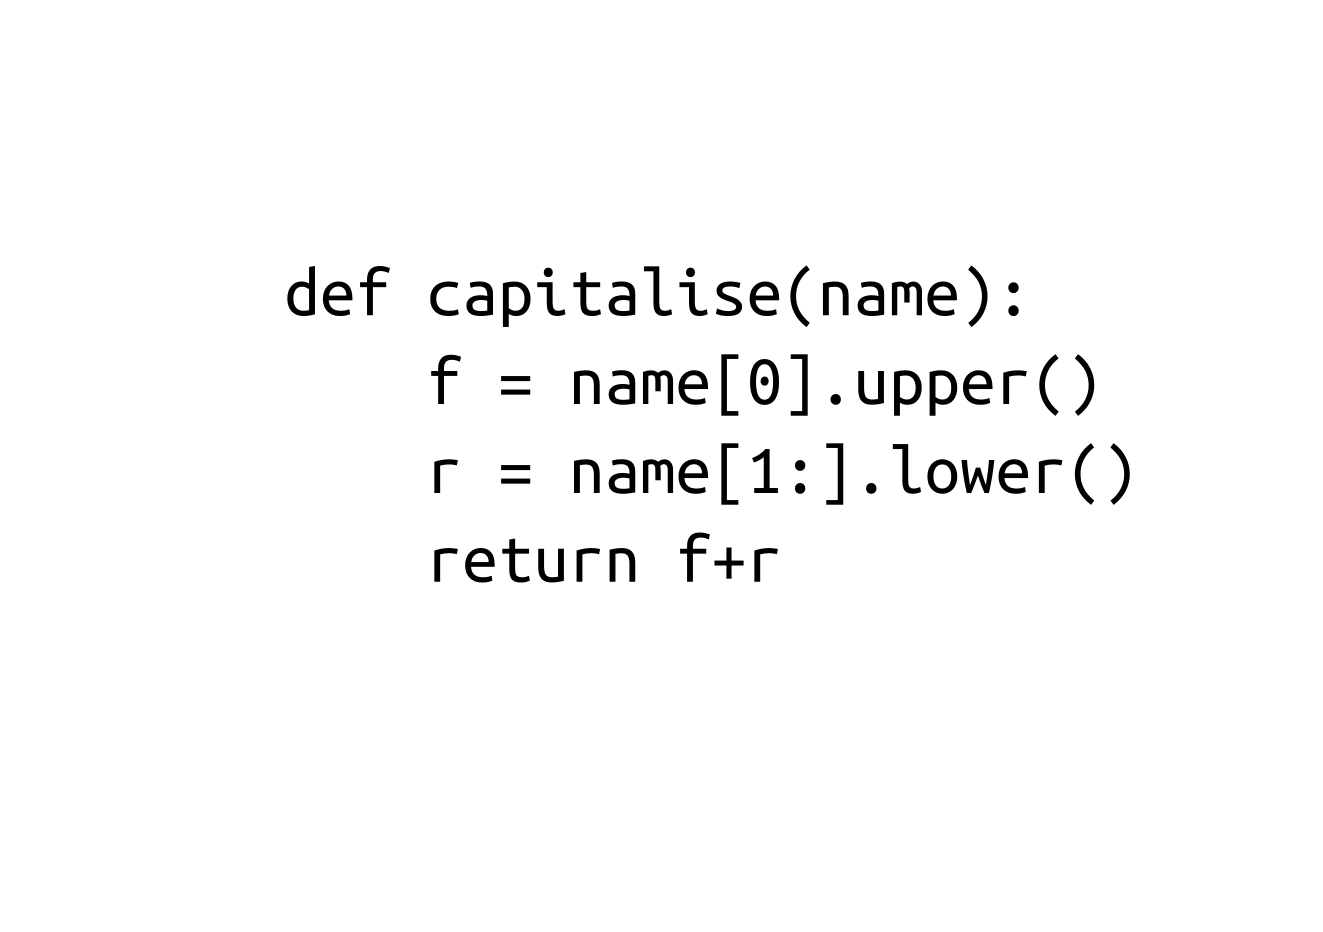
\includegraphics[width=0.9\textwidth]{images/python-code-01.png}

\end{frame}

\begin{frame}{}{}

    \centering
    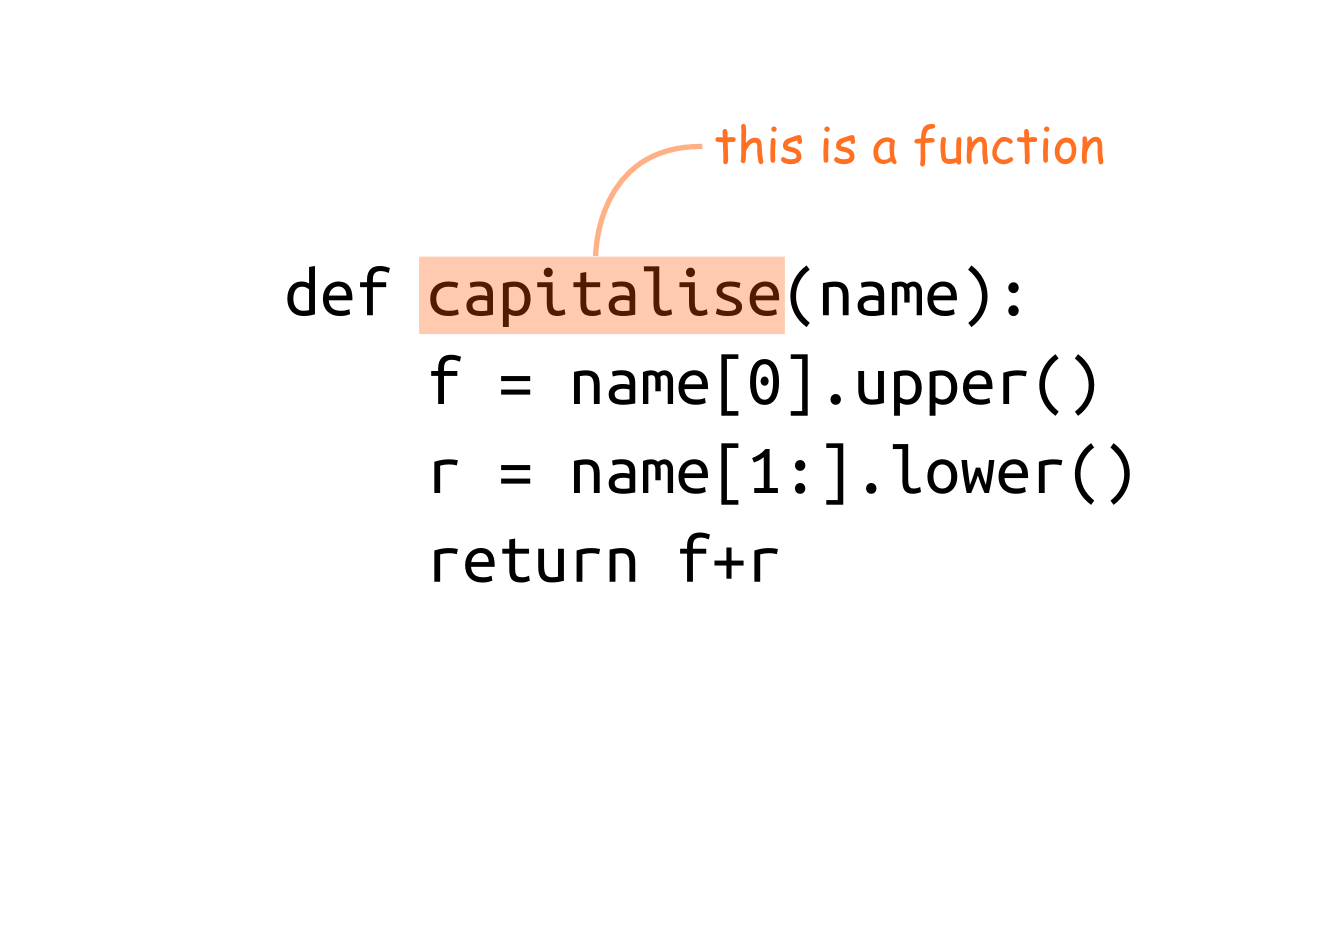
\includegraphics[width=0.9\textwidth]{images/python-code-02.png}

\end{frame}

\begin{frame}{}{}

    \centering
    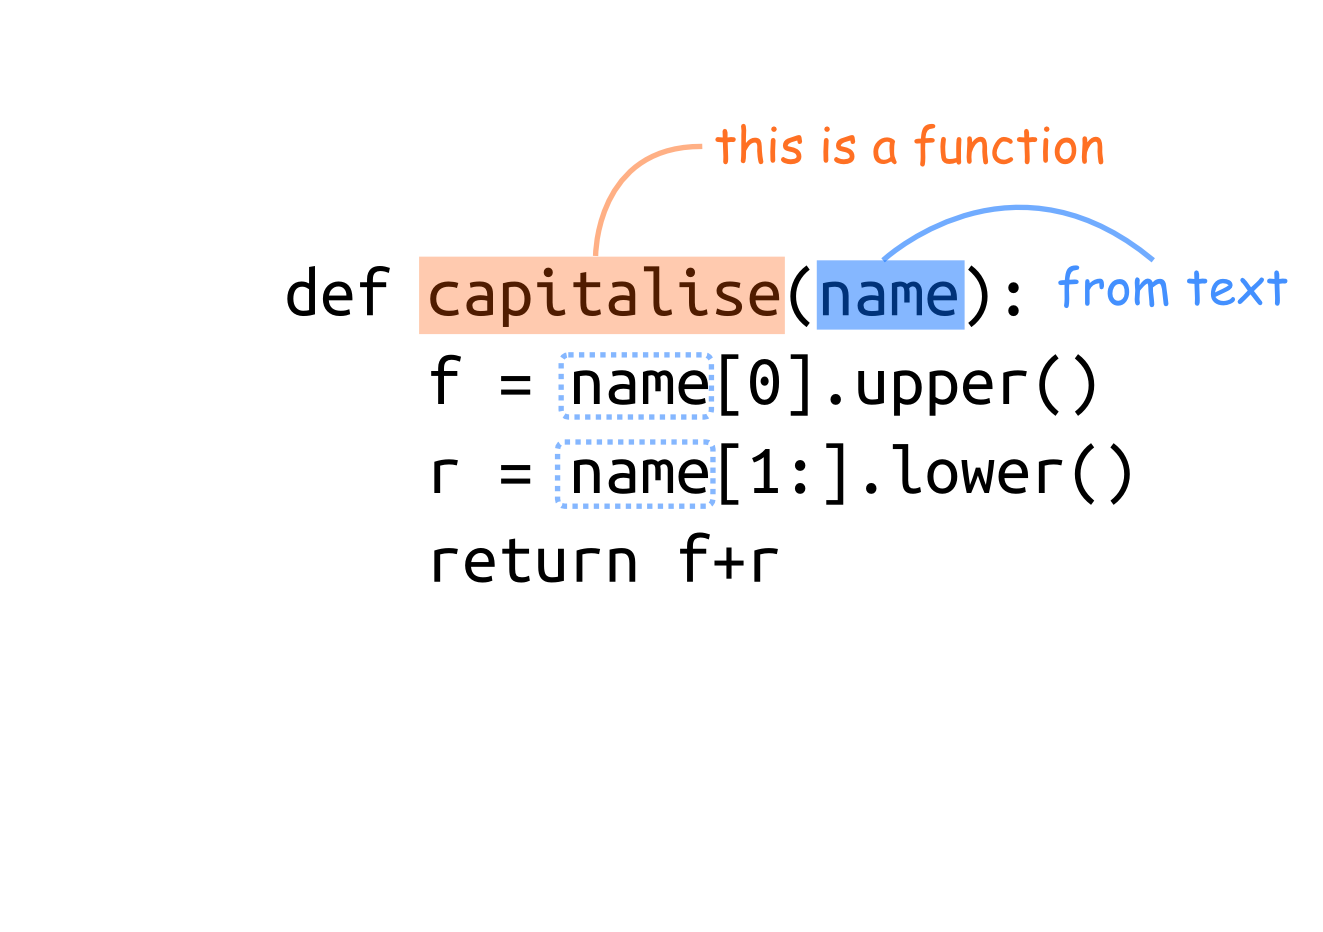
\includegraphics[width=0.9\textwidth]{images/python-code-03.png}

\end{frame}

\begin{frame}{}{}

    \centering
    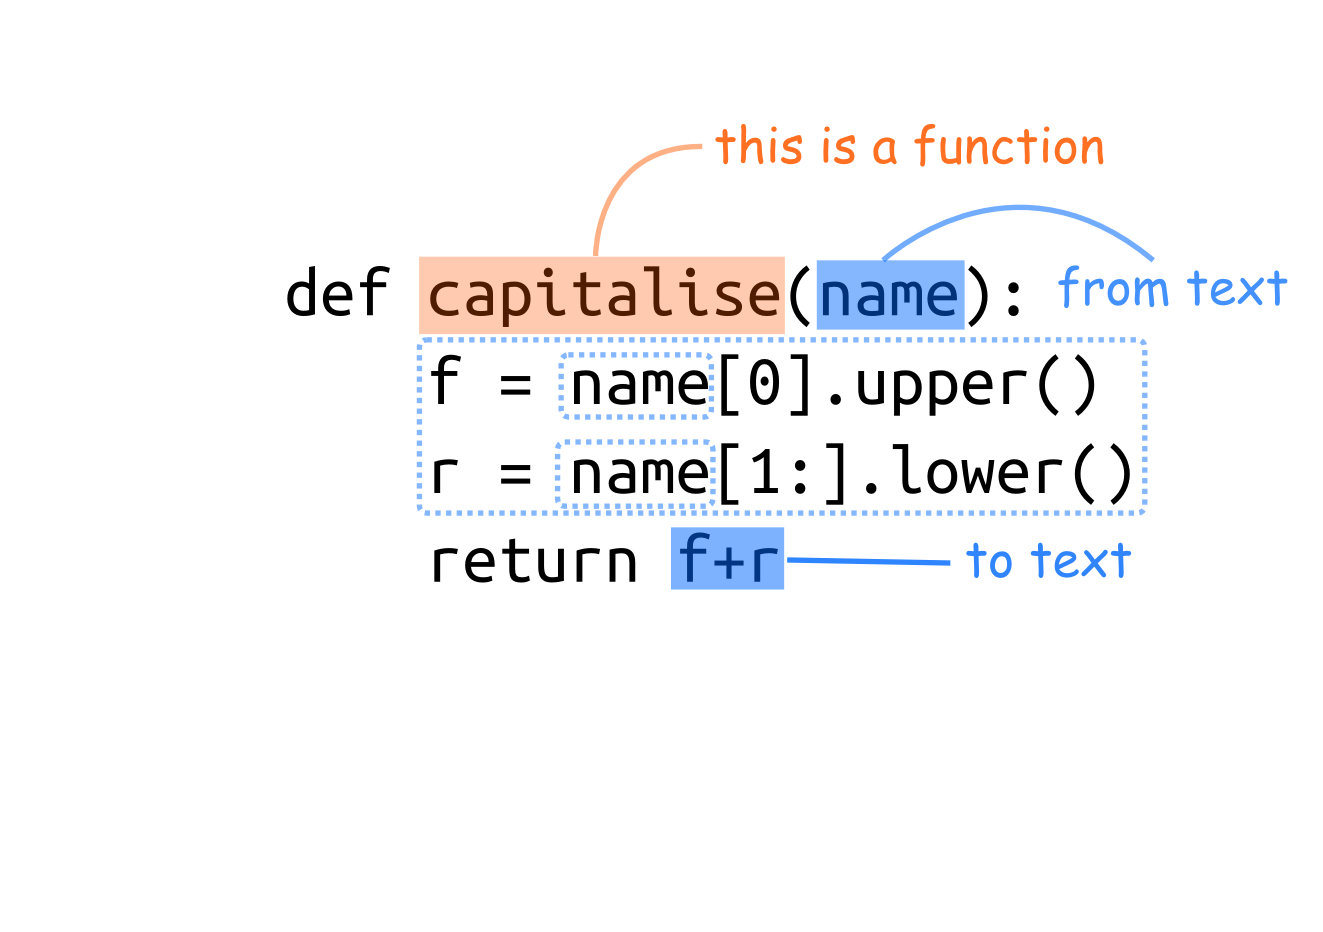
\includegraphics[width=0.9\textwidth]{images/python-code-04.png}

\end{frame}

\begin{frame}{}{}

    \centering
    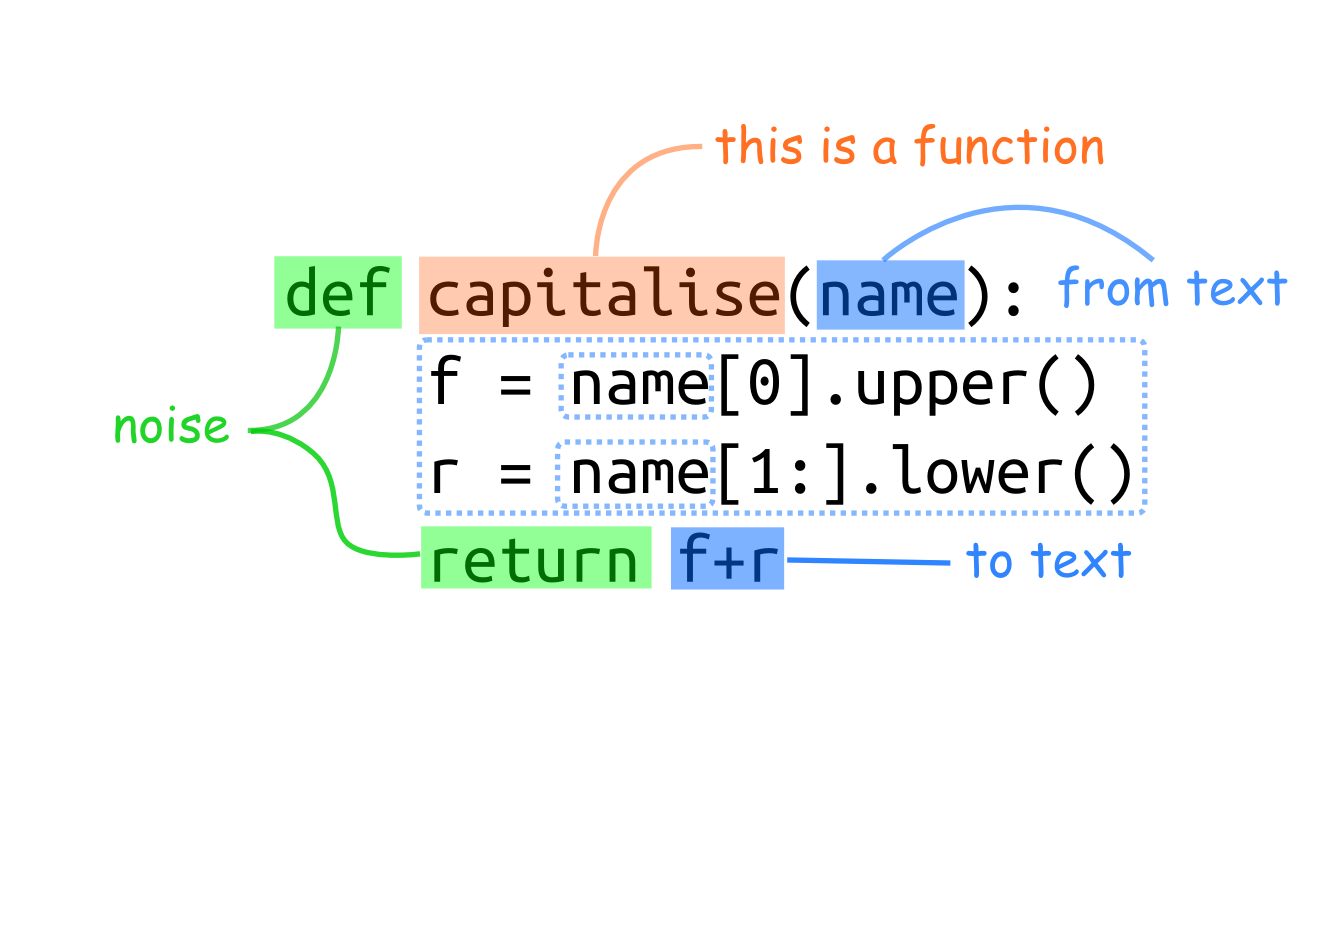
\includegraphics[width=0.9\textwidth]{images/python-code-05.png}

\end{frame}


\begin{frame}{}{}

    \centering
    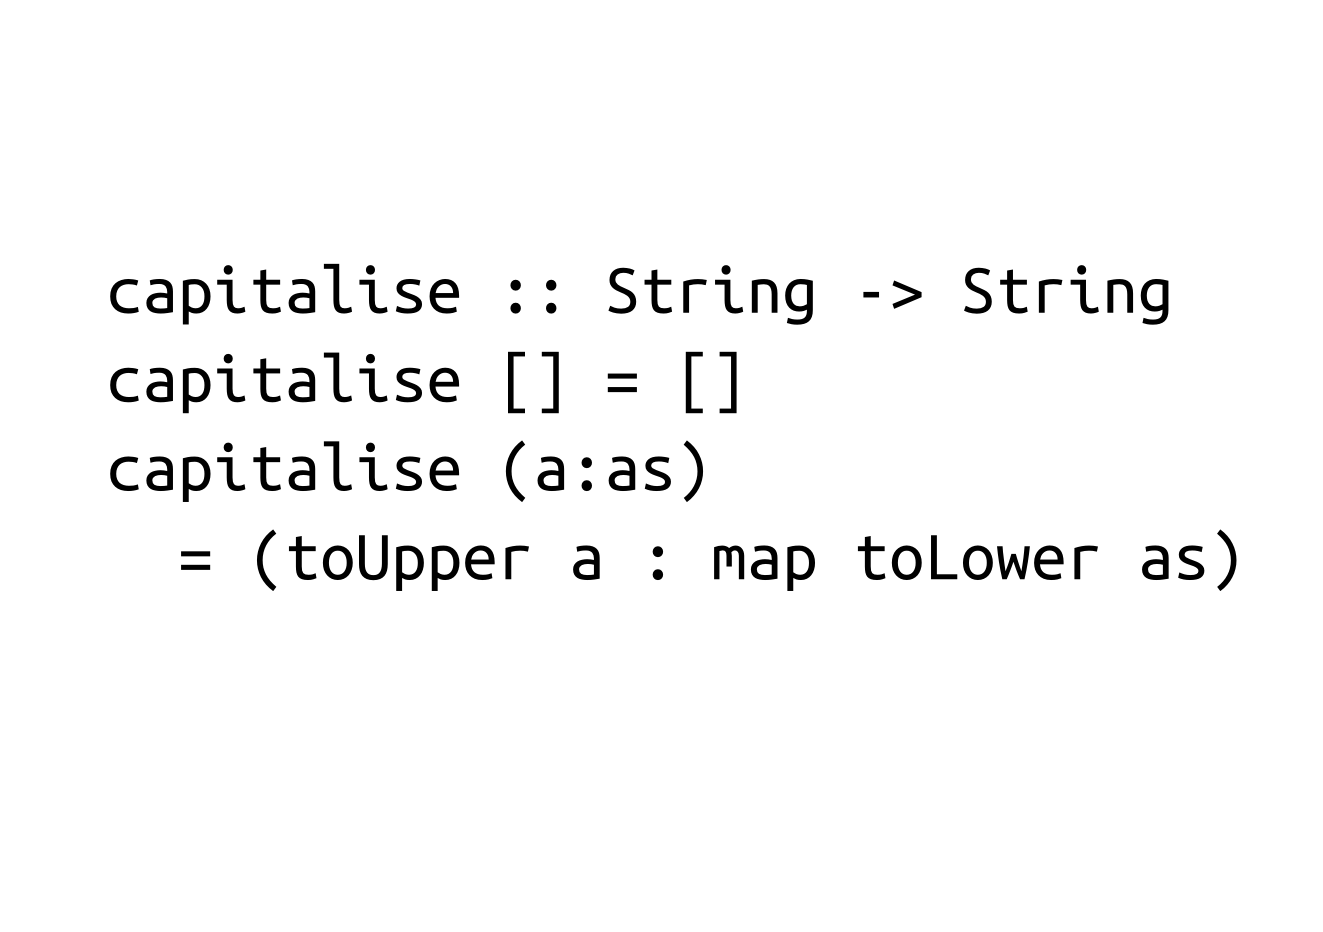
\includegraphics[width=0.9\textwidth]{images/haskell-code-01.png}

\end{frame}

\begin{frame}{}{}

    \centering
    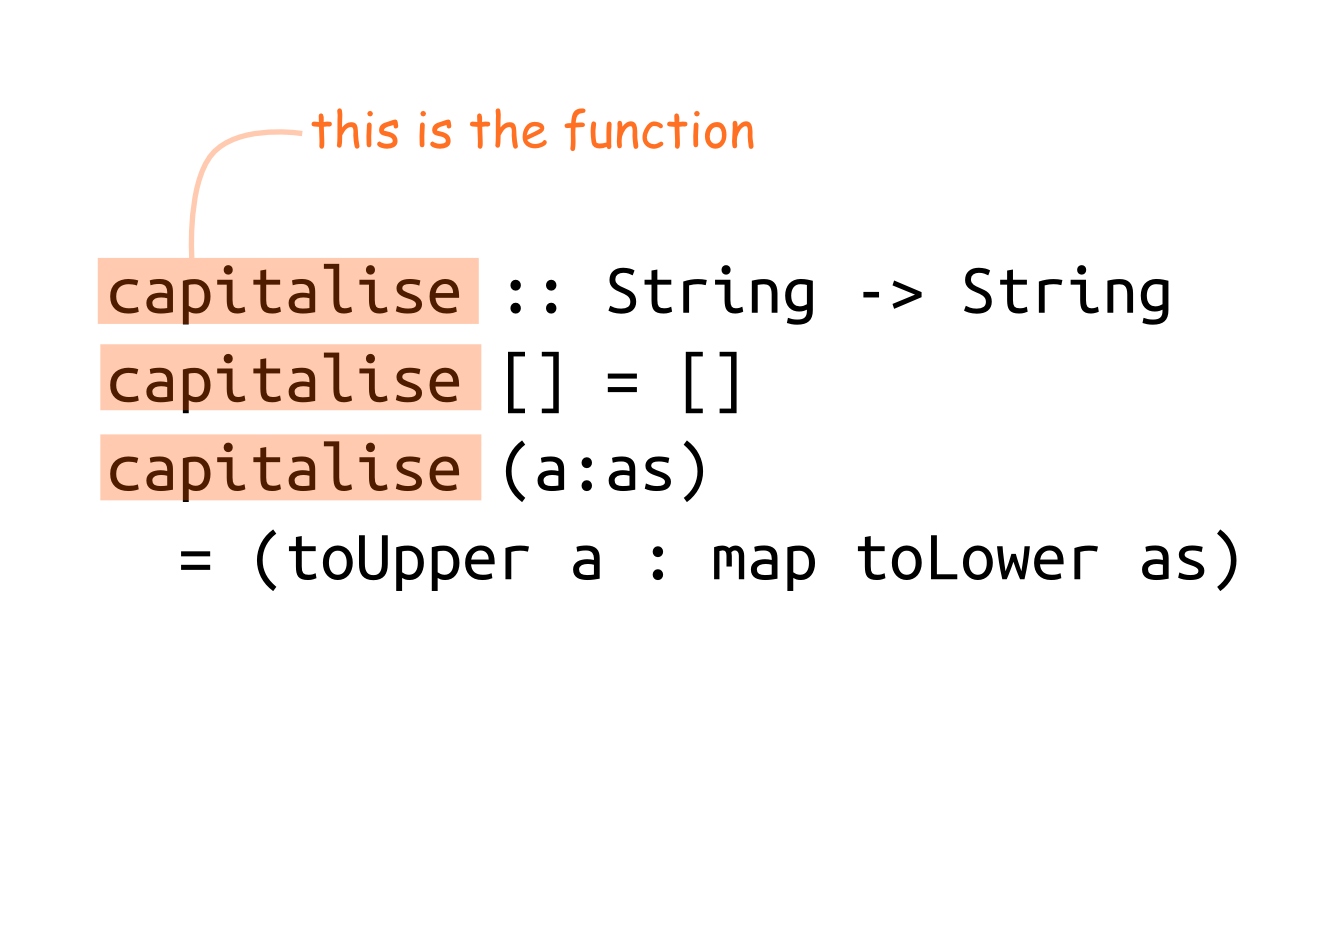
\includegraphics[width=0.9\textwidth]{images/haskell-code-02.png}

\end{frame}

\begin{frame}{}{}

    \centering
    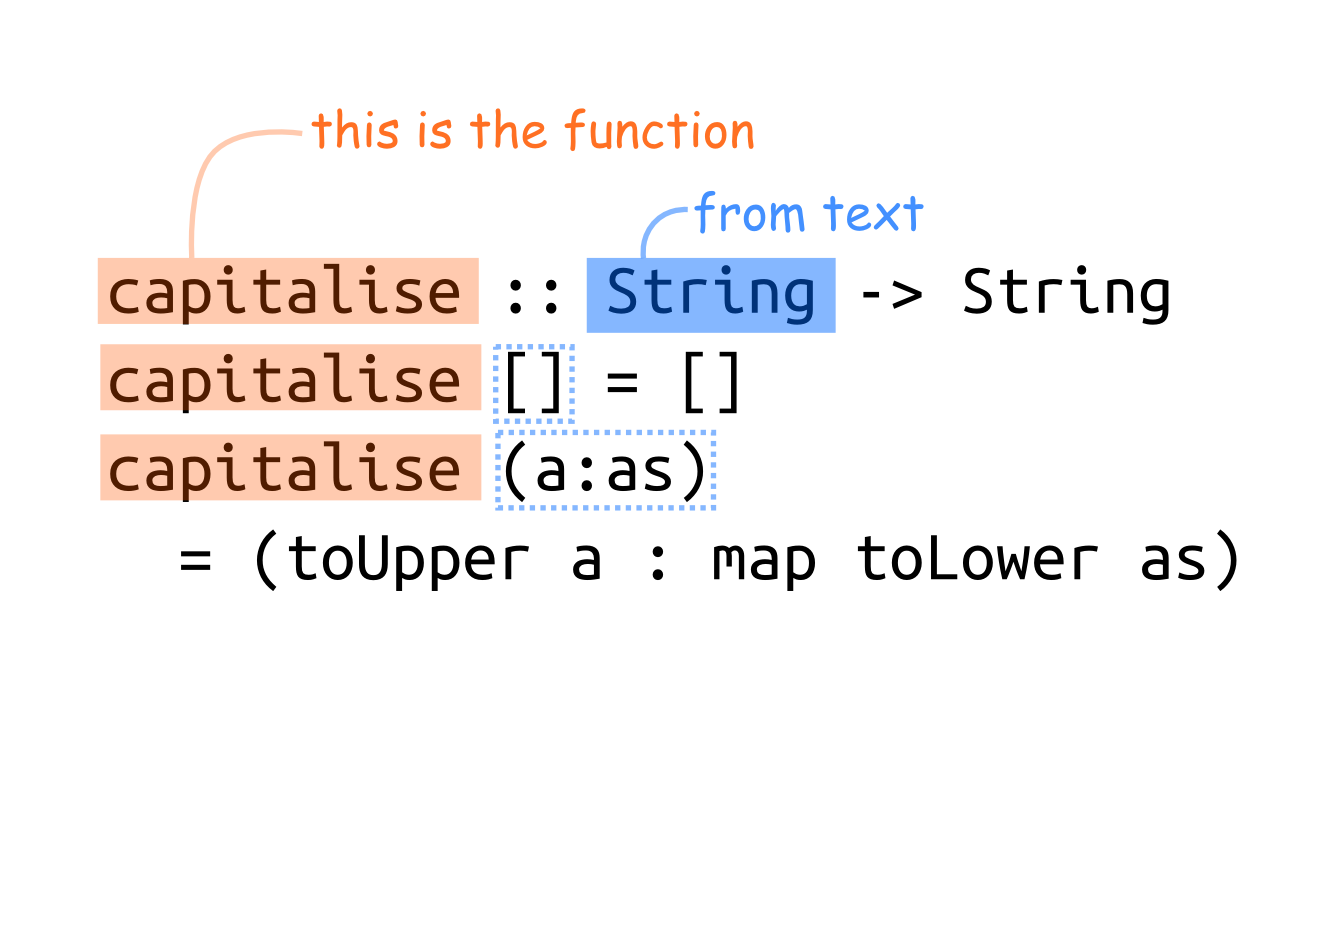
\includegraphics[width=0.9\textwidth]{images/haskell-code-03.png}

\end{frame}

\begin{frame}{}{}

    \centering
    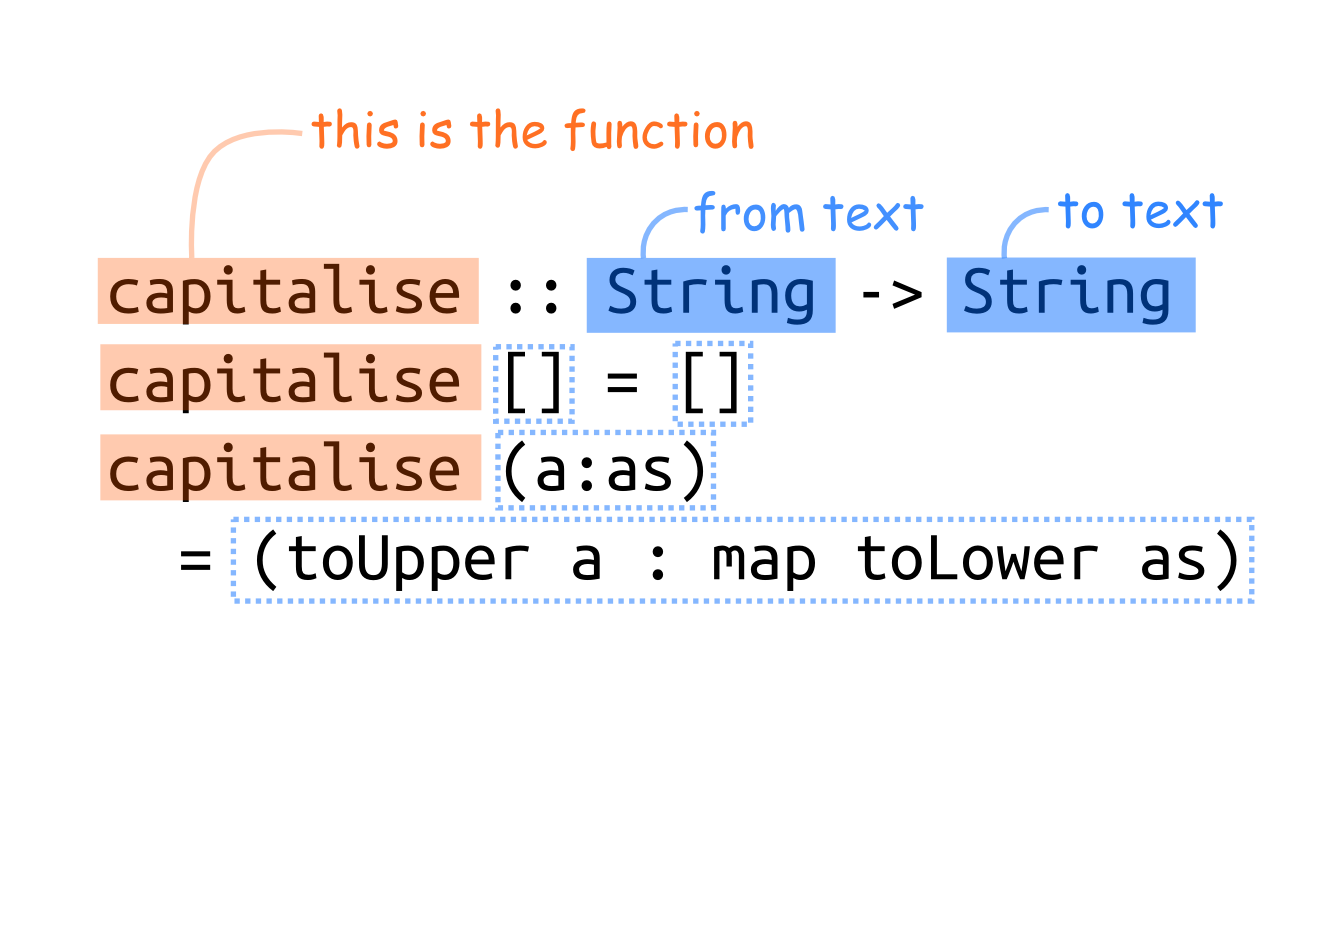
\includegraphics[width=0.9\textwidth]{images/haskell-code-04.png}

\end{frame}

\begin{frame}{}{}

    \centering
    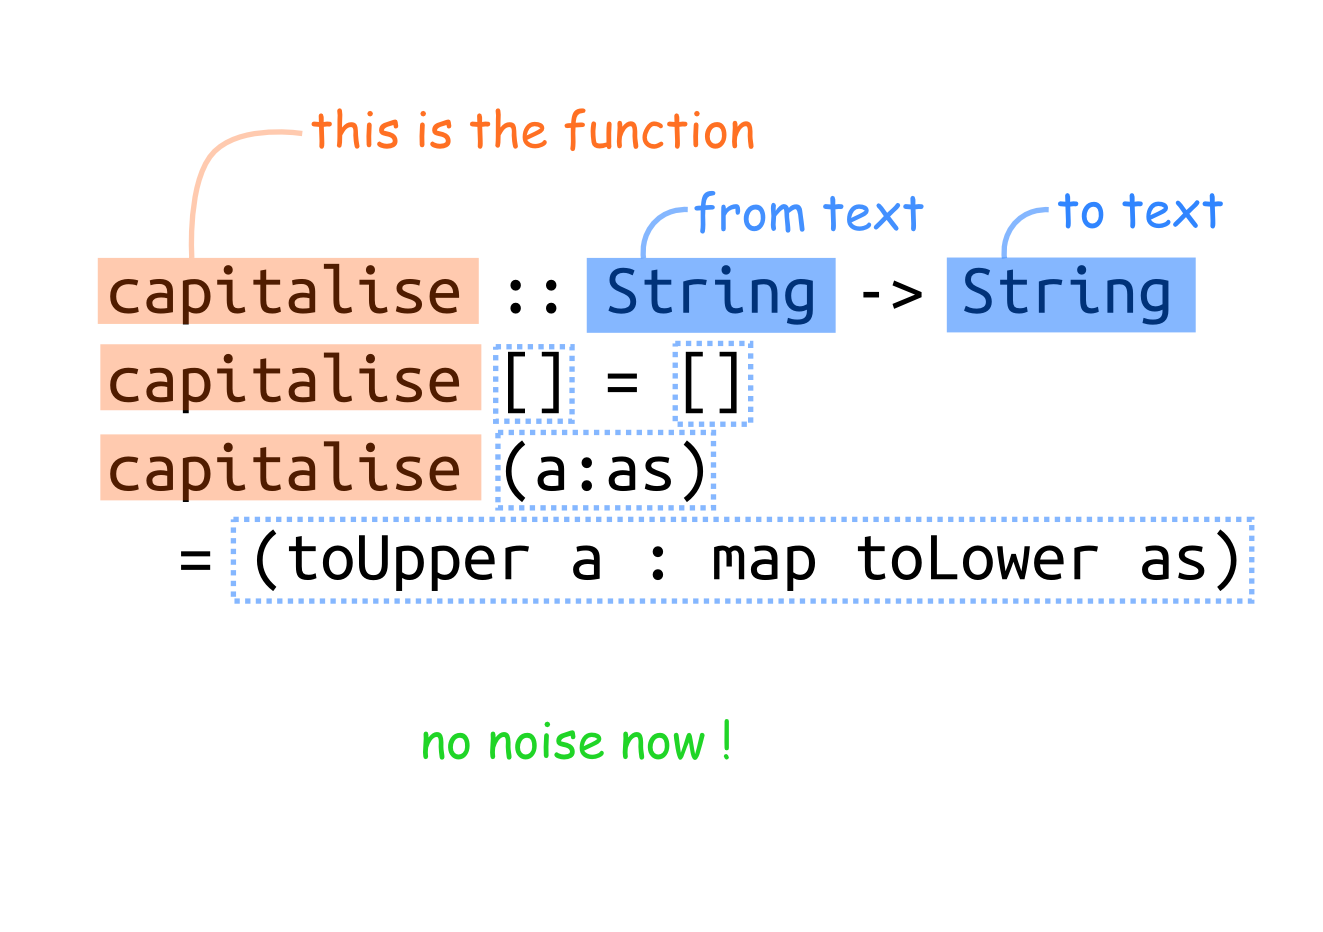
\includegraphics[width=0.9\textwidth]{images/haskell-code-05.png}

\end{frame}


\section{A little category theory}

\begin{frame}{}{}


\end{frame}

\section{Programming patterns}

\begin{frame}{}{}


\end{frame}

\section{Functors}

\begin{frame}{}{}


\end{frame}


\section{Monads}

\begin{frame}{}{}


\end{frame}



\end{document}
